\section{The mean value theorem}
\begin{lemma}[The extreme value theorem]\label{lemma:MINMAX}
	If a function $f$ is continuous on the finite interval $[a,b]$, then there exists $A,B\in[a,b]\ni f(A)\leq f(x)\leq f(B)\,\forall x\in[a,b]$.
	Thus, at the points $A$ and $B$, $f$ has an absolute minimum $m=f(A)$ and an absolute maximum $M=f(B)$.
\end{lemma}
\begin{lemma}[Rolle's theorem]\label{lemma:ROLLES}
	If a function $f$ is continuous on the interval $[a,b]$ and differentiable on $(a,b)$, and $f(a)=f(b)$, then $\exists\,c\in(a,b)\ni f'(c)=0$.
	\begin{proof}
		Consider two cases:
		
		\textbf{Case 1: $f$ remains constant over $[a,b]$}\newline
		If $f(x)=f(a)=f(b)\,\forall x\in(a,b)$, then $f'(x)=0$, and the theorem holds trivially. 
		
		\textbf{Case 2: $f$ is not constant over $[a,b]$}\newline
		If $f$ is not constant over $[a,b]$ and $f(a)=f(b)$, then \lemmaref{lemma:MINMAX} asserts that there must exist an absolute maximum
		or minimum that occur at some point $\eta\in(a,b)$. Since $f$ is differentiable over $(a,b)$, then any point $\eta$ where an absolute
		extremum occurs must also be a local extremum. Consider the case where $\eta$ is a local maxima (the proof for the case of local minima
		is analogous). Then let the interval $I=(\eta-\delta,\eta+\delta)$ for some $\delta>0\ni\forall X\in I,f(X)\leq f(\eta)$.

		Let $h<0$ be a number sufficiently small such that $\eta+h\in I$. $f(\eta+h)\leq f(\eta)\implies f(\eta+h)-f(\eta)\leq0$. Thus,
		$$
			\frac{f(\eta+h)-f(\eta)}{h}\geq0\because\left\{\begin{matrix}
				f(\eta+h)-f(\eta)&\leq0\\
				h&\leq0
			\end{matrix}\right.
		$$
		Taking the left-hand limit as $h\rightarrow0$,
		$$
			\lim_{h\rightarrow0^-}\frac{f(\eta+h)-f(\eta)}{h}=f'(\eta)
		$$
		Now let $H>0$ be a number sufficiently small such that $\eta-H\in I$.
		\begin{align*}
			\frac{f(\eta+H)-f(\eta)}{H}&\leq0\because\left\{\begin{matrix}
				f(\eta+H)-f(\eta)&\leq0\\
				H&\geq0
			\end{matrix}\right.\\
			\lim_{H\rightarrow0^+}\frac{f(\eta+H)-f(\eta)}{H}&=f'(\eta)
		\end{align*}
		Thus,
		\begin{align*}
			0\geq\lim_{H\rightarrow0^+}\frac{f(\eta+H)-f(\eta)}{H}=&f'(\eta)=\lim_{h\rightarrow0^-}\frac{f(\eta+h)-f(\eta)}{h}\geq0\\
			\therefore\,&f'(\eta)=0
		\end{align*}
		Since the same would apply for local minima, then for any local extrema $\eta\in(a,b)$, of which \lemmaref{lemma:MINMAX} asserts
		there must exist at least one, $f'(\eta)=0$.
	\end{proof}
\end{lemma}
\begin{lemma}[The mean value theorem]\label{lemma:MVT}
	For any function $f$ continuous on the interval $[a,b]$ and differentiable on the interval $(a,b)$,
	$\exists\,c\in(a,b)\ni$
	\begin{equation}\label{equation:MVT}
		f'(c)=\frac{f(b)-f(a)}{b-a}
	\end{equation}
	\begin{proof}
		Consider the region of some function $f$ on the finite interval $[a,b]$ over which $f$ is continuous and differentiable over $(a,b)$.
		Let the function $L$ represent the straight line between the points $\point{a}{f(a)}$ and $\point{a}{f(b)}$, given by the expression:
		$$
			L(x)=f(a)+\frac{f(b)-f(a)}{b-a}(x-a)
		$$
		Now consider the function $g$, defined as the difference between $f$ and $L$:
		$$
			g(x)=L(x)-f(x)=f(a)+\frac{f(b)-f(a)}{b-a}(x-a)-f(x)
		$$
		\begin{center}			
			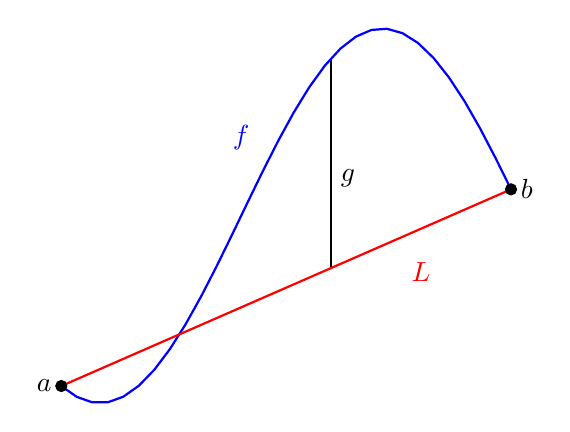
\begin{tikzpicture}
				\begin{axis}
				[
					hide axis,
					domain=-4:4
				]
				\draw[color=black, thick] (1, -0.2790) -- (1, 0.8415);
				\addplot[samples=30, color=blue, thick, domain=-2:3] { sin(deg(x)) };
				\addplot[samples=2, color=red, thick, domain=-2:3] { sin(deg(-2))+(sin(deg(3))-sin(deg(-2)))/5*(x+2) };
				\node[color=black, anchor=west] at (1, 0.2) { $g$ };
				\node[color=blue, anchor=south] at (0, 0.3) { $f$ };
				\node[color=red, anchor=north] at (2, -0.2) { $L$ };
				\filldraw[black] (3, 0.1411) circle (2pt) node[anchor=west] {$b$};
				\filldraw[black] (-2, -0.9093) circle (2pt) node[anchor=east] {$a$};
				\end{axis}
			\end{tikzpicture}
		\end{center}
		Computing the derivative of $g$ with respect to $x$ gives:
		$$
			g'(x)=\frac{f(b)-f(a)}{b-a}-f'(x)
		$$
		Since $g(a)=g(b)=0$, \lemmaref{lemma:ROLLES} asserts that there is some point $c\in(a,b)\st g'(c)=0.$ Thus, at $c$,
		\begin{align*}
			0=g'(c)&=\frac{f(b)-f(a)}{b-a}-f'(c)\\
			\implies f'(c)&=\frac{f(b)-f(a)}{b-a}
		\end{align*}
	\end{proof}
\end{lemma}

\section{Vector calculus}
\subsection{The fundamentals of vector calculus}

\begin{defn}
	\definedterm{Partial derivatives} are an extension of single-variable derivatives in which all variables save
	the one being differentiated by are treated as constants \cite{MORTIMER201389}. A formal definition of the
	partial derivative of some function $f$ with respect to a parameter $x_n$ can be expressed as:
	\begin{equation}
		\pdv{f}{x_n}=\lim_{\delta\rightarrow0}\frac{f(x_1,x_2,\cdots,x_n+\delta,\cdots)-f(x_1,x_2,\cdots,x_n,\cdots)}{\delta}
	\end{equation}
	Partial derivatives allow for the analysis of how multi-variable functions such as scalar- or vector fields change
	with respect to just one spatial dimension. For example, consider the function $f(x,y)=x^2y+\sin(x)\sin y$:
	\begin{align*}
		\pdv{f}{x}=2xy+\cos(x)\sin y&&\pdv{f}{y}=x^2+\sin(x)\cos y
	\end{align*}
	$n$-th order partial derivatives are denoted, similarly to normal calculus, as
	$$
	\pdv[n]{f}{x}=\underbrace{\pdv{x}\cdots\pdv{x}\pdv{f}{x}}_{n\text{ times}}
	$$
\end{defn}
\begin{defn}
	\definedterm{Mixed partial derivatives} are partial derivatives of a function taken with respect to multiple
	variables \cite{GARRETT2015377}. This is denoted as
	$$
	\pdv{f}{\alpha}{\beta}\equiv\pdv{\beta}\pdv{f}{\alpha}
	$$
	where both $\alpha$ and $\beta$ are parameters of $f$.
\end{defn}
\begin{lemma}[Clairaut's theorem]
	Let $f(\alpha,\beta)$ be a function of two parameters $\alpha$ and $\beta$. If the mixed partial derivatives $\pdv{f}{\alpha}{\beta}$
	and $\pdv{f}{\beta}{\alpha}$ exist and are continuous in the open disk $\disk{\alpha_0}{\beta_0}$ centred at
	$\point{\alpha_0}{\beta_0}$ with radius $\delta>0$, then
	$$
		\eval{\pdv{f}{\alpha}{\beta}}_{\point{\alpha_0}{\beta_0}}=\eval{\pdv{f}{\beta}{\alpha}}_{\point{\alpha_0}{\beta_0}}
	$$
	\cite{GARRETT2015377}
	\begin{proof}
		Let $\point{\alpha_0}{\beta_0}$ and $\point{\alpha_1}{\beta_1}$ be points in the domain of $f$. Consider a rectangular region bound by the
		points $W\point{\alpha_0}{\beta_0},X\point{\alpha_1}{\beta_0}, Y\point{\alpha_1}{\beta_1}$  and $Z\point{\alpha_0}{\beta_1}$. 
		$\pdv{f}{\alpha}$ and $\pdv{f}{\beta}$ exist in a neighbourhood of this rectangle, and the mixed partial derivatives 
		$\pdv{f}{\beta}{\alpha}$ and $\pdv{f}{\alpha}{\beta}$ exist and are continuous in this neighbourhood. Let $Q$ be such that
		$$
		Q=[f(\alpha_1,\beta_1)-f(\alpha_0,\beta_1)]-[f(\alpha_1,\beta_0)-f(\alpha_0,\beta_0)]
		$$
		According to the mean value theorem (MVT) $\exists\,\xi_0,\xi_1\in[\alpha_0,\alpha_1]\ni$
		\begin{align*}
			\eval{\pdv{f}{\alpha}}_{\point{\xi_0}{\beta_0}}&=\frac{f(\alpha_1,\beta_0)-f(\alpha_0,\beta_0)}{\alpha_1-\alpha_0}\\
			\eval{\pdv{f}{\alpha}}_{\point{\xi_1}{\beta_1}}&=\frac{f(\alpha_1,\beta_1)-f(\alpha_0,\beta_1)}{\alpha_1-\alpha_0}
		\end{align*}
		Thus $Q$ can be expressed as
		\begin{align*}
			Q&=\left(\eval{\pdv{f}{\alpha}}_{\point{\xi_0}{\beta_0}}\left(\alpha_1-\alpha_0\right)\right)-\left(\eval{\pdv{f}{\alpha}}_{\point{\xi_1}{\beta_1}}\left(\alpha_1-\alpha_0\right)\right)\\
			&=\left(\eval{\pdv{f}{\alpha}}_{\point{\xi_0}{\beta_0}}-\eval{\pdv{f}{\alpha}}_{\point{\xi_1}{\beta_1}}\right)\left(\alpha_1-\alpha_0\right)
		\end{align*}
		Now let $R$ be the equivalent of $Q$ in the direction of $\beta$,
		$$
			R=[f(\alpha_1,\beta_1)-f(\alpha_1,\beta_0)]-[f(\alpha_0,\beta_1)-f(\alpha_0,\beta_0)]
		$$
		By the MVT $\exists\,\zeta_0,\zeta_1\in[\beta_0,\beta_1]\ni$
		\begin{align*}
			\eval{\pdv{f}{\beta}}_{\point{\alpha_0}{\zeta_0}}&=\frac{f(\alpha_0,\beta_1)-f(\alpha_0,\beta_0)}{\beta_1-\beta_0}\\
			\eval{\pdv{f}{\beta}}_{\point{\alpha_1}{\zeta_1}}&=\frac{f(\alpha_1,\beta_1)-f(\alpha_1,\beta_0)}{\beta_1-\beta_0}
		\end{align*}
		Thus $R$ can be expressed as
		\begin{align*}
			R&=\left(\eval{\pdv{f}{\beta}}_{\point{\alpha_0}{\zeta_0}}\left(\beta_1-\beta_0\right)\right)-\left(\eval{\pdv{f}{\beta}}_{\point{\alpha_1}{\zeta_1}}\left(\beta_1-\beta_0\right)\right)\\
			&=\left(\eval{\pdv{f}{\beta}}_{\point{\alpha_0}{\zeta_0}}-\eval{\pdv{f}{\beta}}_{\point{\alpha_1}{\zeta_1}}\right)\left(\beta_1-\beta_0\right)
		\end{align*}
		Rearranging $Q$ and $R$,
		\begin{align*}
			Q&=[f(\alpha_1,\beta_1)-f(\alpha_0,\beta_1)]-[f(\alpha_1,\beta_0)-f(\alpha_0,\beta_0)]\\
			&=f(\alpha_1,\beta_1)-f(\alpha_1,\beta_0)-f(\alpha_0,\beta_1)+f(\alpha_0,\beta_0)\\
			&=[f(\alpha_1,\beta_1)-f(\alpha_1,\beta_0)]-[f(\alpha_0,\beta_1)-f(\alpha_0,\beta_0)]=R\\
			\therefore Q&=R
		\end{align*}
		Thus
		\begin{align}
			\notag\left(\eval{\pdv{f}{\alpha}}_{\point{\xi_0}{\beta_0}}-\eval{\pdv{f}{\alpha}}_{\point{\xi_1}{\beta_1}}\right)\left(\alpha_1-\alpha_0\right)&=\left(\eval{\pdv{f}{\beta}}_{\point{\alpha_0}{\zeta_0}}-\eval{\pdv{f}{\beta}}_{\point{\alpha_1}{\zeta_1}}\right)\left(\beta_1-\beta_0\right)\\
			\label{proof:SYMMETRY}\leadsto\frac{\eval{\pdv*{f}{\alpha}}_{\point{\xi_0}{\beta_0}}-\eval{\pdv*{f}{\alpha}}_{\point{\xi_1}{\beta_1}}}{\beta_1-\beta_0}&=\frac{\eval{\pdv*{f}{\beta}}_{\point{\alpha_0}{\zeta_0}}-\eval{\pdv*{f}{\beta}}_{\point{\alpha_1}{\zeta_1}}}{\alpha_1-\alpha_0}
		\end{align}
		Applying the MVT again $\exists\,\xi^\star\in(\xi_0,\xi_1),\beta^\star\in(\beta_0,\beta_1)\ni$
		\begin{align*}
			\eval{\pdv{f}{\alpha}{\beta}}_{\point{\xi^\star}{\beta^\star}}&=\frac{\eval{\pdv*{f}{\alpha}}_{\point{\xi_1}{\beta_1}}-\eval{\pdv*{f}{\alpha}}_{\point{\xi_0}{\beta_0}}}{\beta_1-\beta_0}\\
			\implies-\eval{\pdv{f}{\alpha}{\beta}}_{\point{\xi^\star}{\beta^\star}}&=\frac{\eval{\pdv*{f}{\alpha}}_{\point{\xi_0}{\beta_0}}-\eval{\pdv*{f}{\alpha}}_{\point{\xi_1}{\beta_1}}}{\beta_1-\beta_0}
		\end{align*}
		Similarly, $\exists\,\alpha^\star\in(\alpha_0,\alpha_1),\zeta^\star\in(\zeta_0,\zeta_1)\ni$
		\begin{align*}
			\eval{\pdv{f}{\beta}{\alpha}}_{\point{\alpha^\star}{\zeta^\star}}&=\frac{\eval{\pdv*{f}{\beta}}_{\point{\alpha_1}{\zeta_1}}-\eval{\pdv*{f}{\beta}}_{\point{\alpha_0}{\zeta_0}}}{\alpha_1-\alpha_0}\\
			\implies-\eval{\pdv{f}{\beta}{\alpha}}_{\point{\alpha^\star}{\zeta^\star}}&=\frac{\eval{\pdv*{f}{\beta}}_{\point{\alpha_0}{\zeta_0}}-\eval{\pdv*{f}{\beta}}_{\point{\alpha_1}{\zeta_1}}}{\alpha_1-\alpha_0}
		\end{align*}
		Substituting back into \eqref{proof:SYMMETRY},
		\begin{align*}
			-\eval{\pdv{f}{\alpha}{\beta}}_{\point{\xi^\star}{\beta^\star}}&=-\eval{\pdv{f}{\beta}{\alpha}}_{\point{\alpha^\star}{\zeta^\star}}\\
			\implies\eval{\pdv{f}{\alpha}{\beta}}_{\point{\xi^\star}{\beta^\star}}&=\eval{\pdv{f}{\beta}{\alpha}}_{\point{\alpha^\star}{\zeta^\star}}
		\end{align*}
		Consequently, as $\alpha_1\rightarrow\alpha_0$ and $\beta_1\rightarrow\beta_0$, $\xi^\star\rightarrow\alpha_0,\beta^\star\rightarrow\beta_0,\alpha^\star\rightarrow\alpha_0$ 
		and $\zeta^\star\rightarrow\beta_0$. Since the derivatives are continuous,
		$$
			\eval{\pdv{f}{\beta}{\alpha}}_{\point{\alpha_0}{\beta_0}}=\eval{\pdv{f}{\alpha}{\beta}}_{\point{\alpha_0}{\beta_0}}
		$$
		Because $\point{\alpha_0}{\beta_0}$ is an arbitrary point in the domain, $\pdv{f}{\beta}{\alpha}=\pdv{f}{\alpha}{\beta}$ at 
		all points in the domain where the mixed partial derivatives are continuous.
	\end{proof}
\end{lemma}
\begin{defn}
	The \definedterm{nabla} operator $\nabla$ is a vector containing one partial derivative for each parameter of
	the function applied to \cite{RAPP2017137}. For some function $f:\mathbb{R}^n\rightarrow\mathbb{R}$, $\nabla f$ would be given by:
	$$
	\nabla f=\begin{bmatrix}
		\pdv*{f}{x_1}\\
		\pdv*{f}{x_2}\\
		\vdots\\
		\pdv*{f}{x_n}
	\end{bmatrix}
	$$
\end{defn}
\begin{defn}
	The directional derivative in the direction of some vector $\vec{v}$ of the function $f$ which is differentiable in
	the open disk $\disk{x_0}{y_0}$ centred at $\point{x_0}{y_0}$ with radius $\delta>0$ is defined as
	$$
		\eval{\nabla_{\vec{v}}f\,}_{\point{x_0}{y_0}}=\frac{\eval{\nabla f}_{\point{x_0}{y_0}}\cdot\vec{v}}{\lVert\vec{v}\rVert}
	$$
	\cite{GIANNAKIDIS2010129}
\end{defn}